\documentclass[aspectratio=169,10pt]{beamer}

\usetheme{Madrid}
\usecolortheme{default}
\setbeamertemplate{navigation symbols}{}
\setbeamertemplate{footline}[frame number]

\usepackage[T1]{fontenc}
\usepackage[utf8]{inputenc}
\usepackage{lmodern}
\usepackage{booktabs}
\usepackage{array}
\usepackage{tikz}
\usepackage{graphicx}
\usepackage{multicol}
\usepackage{amsmath}
\usetikzlibrary{arrows.meta,positioning,shapes.geometric,calc,fit}

\definecolor{AccentBlue}{HTML}{1F4E79}
\definecolor{AccentTeal}{HTML}{0F766E}
\definecolor{AccentOrange}{HTML}{C2410C}
\definecolor{SoftGray}{HTML}{EEF2F7}
\definecolor{DarkGray}{HTML}{334155}
\definecolor{Placeholder}{HTML}{64748B}

\setbeamercolor{title}{fg=AccentBlue}
\setbeamercolor{frametitle}{fg=AccentBlue}
\setbeamercolor{structure}{fg=AccentBlue}
\setbeamercolor{block title}{fg=white,bg=AccentBlue}
\setbeamercolor{block body}{fg=black,bg=SoftGray}
\setbeamerfont{framesubtitle}{size=\small}

\newcommand{\smallnote}[1]{{\footnotesize\color{DarkGray}#1}}

\newcommand{\placeholderbox}[2]{
  \begin{tikzpicture}
    \node[
      draw=Placeholder,
      dashed,
      rounded corners=3pt,
      minimum width=#1,
      minimum height=#2,
      align=center,
      text=Placeholder,
      fill=SoftGray
    ] {Placeholder};
  \end{tikzpicture}
}

\title{Music Genre Classification on FMA Datasets}
\subtitle{61.502 Deep Learning for Enterprise (Y2026)}
\author{Ang Kar Kin \and Nicolas Lasch \and Nisal Jinadasa}
\date{April 2026}

\begin{document}

\begin{frame}[plain]
\begin{tikzpicture}[remember picture,overlay]
  \fill[black!2] (current page.south west) rectangle (current page.north east);
  \foreach \x in {0.7,1.1,...,12.5} {
    \draw[AccentBlue!35, line width=0.5pt]
      ([xshift=\x cm,yshift=0.8cm]current page.south west)
      .. controls +(0,1.4) and +(0,-1.1) ..
      ([xshift=\x cm,yshift=4.0cm]current page.south west);
  }
\end{tikzpicture}
\vspace{0.4cm}
\begin{columns}[T,totalwidth=\textwidth]
\column{0.64\textwidth}
{\usebeamerfont{title}\usebeamercolor[fg]{title}\LARGE\inserttitle\par}
\vspace{0.2cm}
{\large \insertsubtitle\par}
\vspace{0.6cm}
{\normalsize We built a CNN-based audio classification pipeline on FMA-Large, compared model variants under a reproducible protocol, and packaged the result into a working demo flow.\par}
\vspace{0.7cm}
{\small \insertauthor\par}
\vspace{0.1cm}
{\small \insertdate\par}

\column{0.36\textwidth}
\begin{block}{System Overview}
\small
\begin{itemize}
  \item FMA metadata + audio
  \item Mel features + CNN training
  \item Evaluation + demo API
\end{itemize}
\end{block}
\vspace{0.2cm}
\placeholderbox{0.95\linewidth}{1.2cm}
\smallnote{Repo / demo link placeholder}
\end{columns}
\end{frame}

\begin{frame}{Why Genre Classification Matters}
\framesubtitle{The task looks simple, but the labels are subjective and the audio patterns are messy.}
\begin{columns}[T,totalwidth=\textwidth]
\column{0.44\textwidth}
\small
\setlength{\itemsep}{2pt}
\begin{itemize}
  \item Supports playlisting, search, recommendation, and catalog organization.
  \item Manual tagging is expensive and inconsistent at large scale.
  \item Genre labels are proxy labels, not ground truth, so overlap is expected.
  \item Audio varies over time, so short clips may miss the full track identity.
  \item This project treats the task as an end-to-end ML pipeline, not a notebook demo.
\end{itemize}

\column{0.56\textwidth}
\centering
\resizebox{\linewidth}{!}{
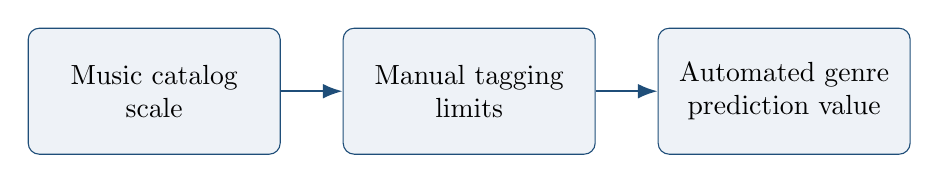
\begin{tikzpicture}[
  box/.style={draw=AccentBlue, rounded corners=4pt, fill=SoftGray, minimum width=3.2cm, minimum height=1.6cm, align=center},
  arr/.style={-{Latex[length=2.5mm]}, thick, AccentBlue}
]
\node[box] (a) at (0,0) {Music catalog\\scale};
\node[box] (b) at (4.0,0) {Manual tagging\\limits};
\node[box] (c) at (8.0,0) {Automated genre\\prediction value};
\draw[arr] (a) -- (b);
\draw[arr] (b) -- (c);
\end{tikzpicture}
}
\vspace{0.3cm}

\smallnote{Framing: useful for retrieval, discovery, and downstream personalization.}
\end{columns}
\end{frame}

\begin{frame}{FMA Family Overview}
\framesubtitle{Two subsets matter here: one as a benchmark, one as the harder scale test.}
\begin{columns}[T,totalwidth=\textwidth]
\column{0.46\textwidth}
\begin{block}{Why Discuss Both?}
\small
\begin{itemize}
  \item FMA-Medium is a standard benchmark subset.
  \item FMA-Large increases label diversity and scale.
  \item Comparing both helps explain why this project chose the harder setup.
\end{itemize}
\end{block}
\smallnote{Source: official FMA dataset release / ISMIR 2017 paper.}

\column{0.54\textwidth}
\centering
\begin{tabular}{>{\raggedright\arraybackslash}p{2.7cm} >{\centering\arraybackslash}p{2.4cm} >{\centering\arraybackslash}p{2.0cm}}
\toprule
Dataset & Tracks & Genres \\
\midrule
FMA-Medium & 25{,}000 & 16 \\
FMA-Large & 106{,}574 & 161 \\
\bottomrule
\end{tabular}
\vspace{0.3cm}

\resizebox{\linewidth}{!}{
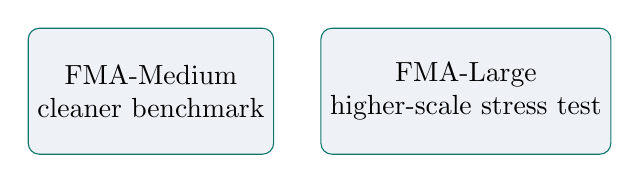
\begin{tikzpicture}[
  card/.style={draw=AccentTeal, rounded corners=4pt, fill=SoftGray, minimum width=2.9cm, minimum height=1.6cm, align=center}
]
\node[card] (m) at (0,0) {FMA-Medium\\cleaner benchmark};
\node[card] (l) at (4.0,0) {FMA-Large\\higher-scale stress test};
\end{tikzpicture}
}
\end{columns}
\end{frame}

\begin{frame}{Why We Train on FMA-Large}
\framesubtitle{The project uses the larger subset so the model must handle more classes and more imbalance.}
\begin{columns}[T,totalwidth=\textwidth]
\column{0.44\textwidth}
\begin{itemize}
  \item FMA-Medium offers a simpler benchmark with fewer classes.
  \item FMA-Large better reflects scale, imbalance, and ambiguity in realistic music catalogs.
  \item This repo trains and evaluates on \texttt{fma\_large} using labels from \texttt{fma\_metadata/tracks.csv}.
  \item The main reported task is single-label top-genre classification.
\end{itemize}

\column{0.56\textwidth}
\centering
\resizebox{\linewidth}{!}{
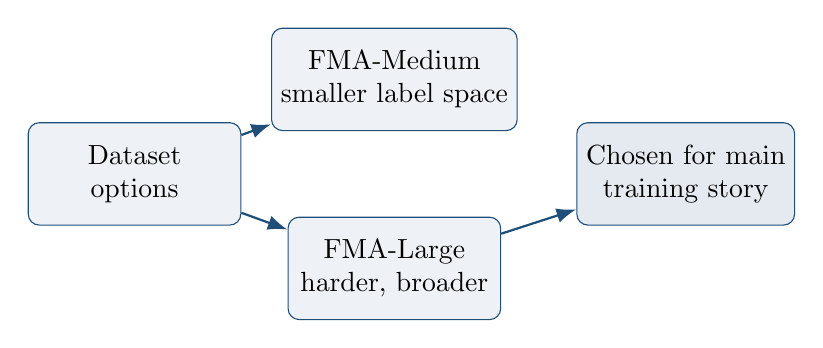
\begin{tikzpicture}[
  box/.style={draw=AccentBlue, rounded corners=4pt, fill=SoftGray, minimum width=2.7cm, minimum height=1.3cm, align=center},
  arr/.style={-{Latex[length=2.5mm]}, thick, AccentBlue}
]
\node[box] (start) at (0,0) {Dataset\\options};
\node[box] (mid1) at (3.3,1.2) {FMA-Medium\\smaller label space};
\node[box] (mid2) at (3.3,-1.2) {FMA-Large\\harder, broader};
\node[box, fill=AccentBlue!12] (end) at (7.0,0) {Chosen for main\\training story};
\draw[arr] (start) -- (mid1);
\draw[arr] (start) -- (mid2);
\draw[arr] (mid2) -- (end);
\end{tikzpicture}
}
\end{columns}
\end{frame}

\begin{frame}{Data Filtering and Split Policy}
\framesubtitle{We keep only trainable audio and preserve a clean evaluation split.}
\begin{columns}[T,totalwidth=\textwidth]
\column{0.43\textwidth}
\begin{itemize}
  \item Keep only \texttt{subset == large} and non-null \texttt{track.genre\_top}.
  \item Exclude missing or known-bad audio where needed.
  \item Use a stratified \texttt{80 / 10 / 10} train/val/test split.
  \item Apply a rare-class support policy before final training.
\end{itemize}
\vspace{0.2cm}
\begin{block}{Main Run Counts}
\small
Labeled valid tracks: \textbf{24,552}\\
Train / Val / Test: \textbf{19,549 / 2,444 / 2,444}\\
Final classes after support policy: \textbf{11}
\end{block}

\column{0.57\textwidth}
\centering
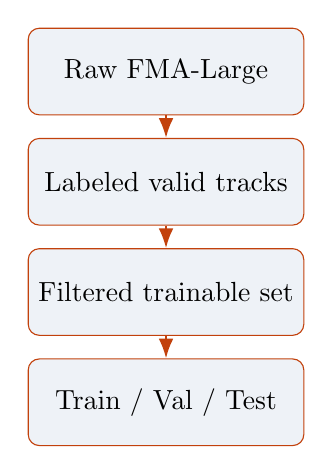
\begin{tikzpicture}[
  stage/.style={draw=AccentOrange, rounded corners=4pt, fill=SoftGray, minimum width=3.5cm, minimum height=1.1cm, align=center},
  arr/.style={-{Latex[length=2.5mm]}, thick, AccentOrange}
]
\node[stage] (a) at (0,0) {Raw FMA-Large};
\node[stage] (b) at (0,-1.4) {Labeled valid tracks};
\node[stage] (c) at (0,-2.8) {Filtered trainable set};
\node[stage] (d) at (0,-4.2) {Train / Val / Test};
\draw[arr] (a) -- (b);
\draw[arr] (b) -- (c);
\draw[arr] (c) -- (d);
\end{tikzpicture}
\vspace{0.2cm}

\smallnote{Support-policy thresholds in the notebook reduce the final label space to 11 classes.}
\end{columns}
\end{frame}

\begin{frame}{End-to-End Pipeline Overview}
\framesubtitle{One consistent pipeline feeds both model training and the demo artifact.}
\centering
\resizebox{\textwidth}{!}{
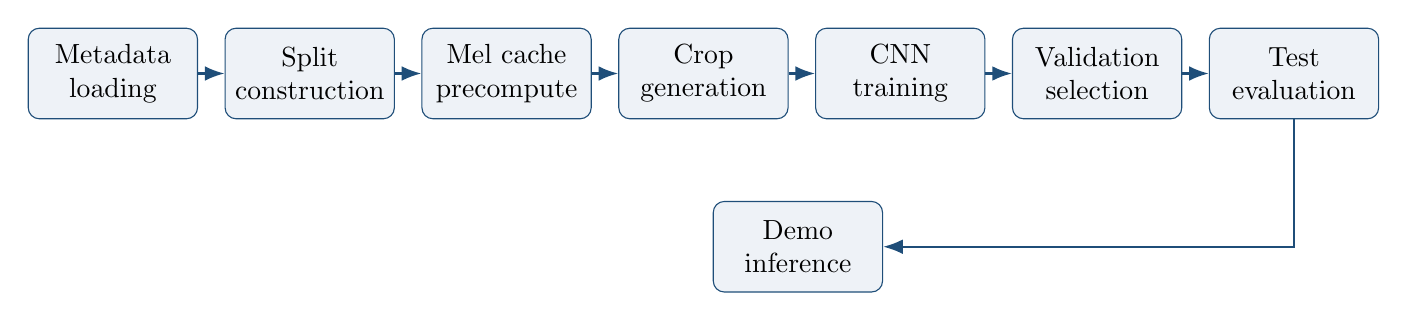
\begin{tikzpicture}[
  x=1cm, y=1cm,
  block/.style={draw=AccentBlue, rounded corners=4pt, fill=SoftGray, minimum width=2.15cm, minimum height=1.15cm, align=center},
  arr/.style={-{Latex[length=2.5mm]}, thick, AccentBlue}
]
\node[block] (a) at (0,0) {Metadata\\loading};
\node[block] (b) at (2.5,0) {Split\\construction};
\node[block] (c) at (5.0,0) {Mel cache\\precompute};
\node[block] (d) at (7.5,0) {Crop\\generation};
\node[block] (e) at (10.0,0) {CNN\\training};
\node[block] (f) at (12.5,0) {Validation\\selection};
\node[block] (g) at (15.0,0) {Test\\evaluation};
\node[block] (h) at (8.7,-2.2) {Demo\\inference};
\draw[arr] (a) -- (b);
\draw[arr] (b) -- (c);
\draw[arr] (c) -- (d);
\draw[arr] (d) -- (e);
\draw[arr] (e) -- (f);
\draw[arr] (f) -- (g);
\draw[arr] (g) |- (h);
\end{tikzpicture}
}

\vspace{0.35cm}
\begin{itemize}
  \item The main training story and the later demo share the same high-level pipeline shape.
  \item The anchor idea is reproducibility: consistent preprocessing, comparable runs, and saved artifacts.
\end{itemize}
\end{frame}

\begin{frame}{Audio Feature Engineering}
\framesubtitle{The model sees spectrograms, not raw waveforms, so the input must be normalized first.}
\begin{columns}[T,totalwidth=\textwidth]
\column{0.46\textwidth}
\small
\begin{itemize}
  \item Audio is standardized to \textbf{22,050 Hz}.
  \item Features use \textbf{128 Mel bins} with \texttt{n\_fft = 2048} and \texttt{hop = 512}.
  \item The pipeline precomputes up to \textbf{29 s} full-track Mel caches.
  \item Training and evaluation use \textbf{5 s} crops for a fixed model input view.
  \item Mel features preserve useful structure while keeping training practical.
\end{itemize}

\column{0.54\textwidth}
\centering
\resizebox{\linewidth}{!}{
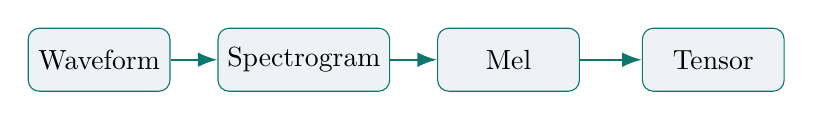
\begin{tikzpicture}[
  box/.style={draw=AccentTeal, rounded corners=4pt, fill=SoftGray, minimum width=1.8cm, minimum height=0.8cm, align=center},
  arr/.style={-{Latex[length=2.5mm]}, thick, AccentTeal}
]
\node[box] (a) at (0,0) {Waveform};
\node[box] (b) at (2.6,0) {Spectrogram};
\node[box] (c) at (5.2,0) {Mel};
\node[box] (d) at (7.8,0) {Tensor};
\draw[arr] (a) -- (b);
\draw[arr] (b) -- (c);
\draw[arr] (c) -- (d);
\end{tikzpicture}
}
\vspace{0.15cm}

\placeholderbox{0.82\linewidth}{0.7cm}
\smallnote{Insert real Mel spectrogram screenshot from notebook}
\end{columns}
\end{frame}

\begin{frame}{Modeling: CNN Variants}
\framesubtitle{We compare a simpler stack against a residual design that trains more reliably.}
\begin{columns}[T,totalwidth=\textwidth]
\column{0.48\textwidth}
\begin{block}{Standard CNN}
\small
\begin{itemize}
  \item Simpler stacked convolution blocks
  \item Baseline and augmentation comparison runs
  \item Lower capacity and weaker stability
\end{itemize}
\end{block}
\centering
\resizebox{\linewidth}{!}{
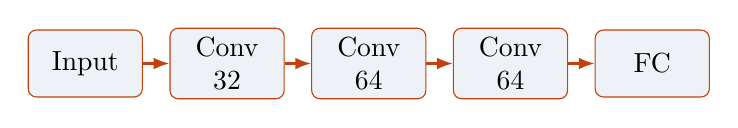
\begin{tikzpicture}[
  box/.style={draw=AccentOrange, rounded corners=3pt, fill=SoftGray, minimum width=1.45cm, minimum height=0.85cm, align=center},
  arr/.style={-{Latex[length=2mm]}, thick, AccentOrange}
]
\node[box] (a) at (0,0) {Input};
\node[box] (b) at (1.8,0) {Conv\\32};
\node[box] (c) at (3.6,0) {Conv\\64};
\node[box] (d) at (5.4,0) {Conv\\64};
\node[box] (e) at (7.2,0) {FC};
\draw[arr] (a) -- (b);
\draw[arr] (b) -- (c);
\draw[arr] (c) -- (d);
\draw[arr] (d) -- (e);
\end{tikzpicture}
}

\column{0.52\textwidth}
\begin{block}{Residual CNN}
\small
\begin{itemize}
  \item Residual blocks improve gradient flow
  \item Strongest model in the saved results
  \item Better optimization stability on the harder setup
\end{itemize}
\end{block}
\centering
\resizebox{\linewidth}{!}{
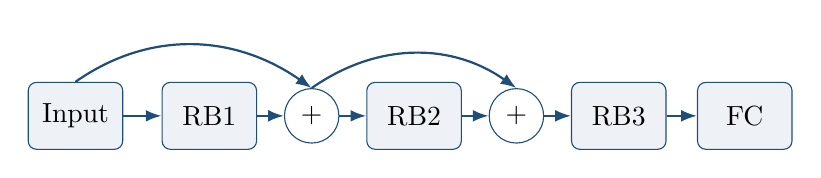
\begin{tikzpicture}[
  box/.style={draw=AccentBlue, rounded corners=3pt, fill=SoftGray, minimum width=1.2cm, minimum height=0.85cm, align=center},
  plus/.style={circle, draw=AccentBlue, minimum size=0.45cm},
  arr/.style={-{Latex[length=2mm]}, thick, AccentBlue}
]
\node[box] (a) at (0,0) {Input};
\node[box] (b) at (1.7,0) {RB1};
\node[plus] (p1) at (3.0,0) {$+$};
\node[box] (c) at (4.3,0) {RB2};
\node[plus] (p2) at (5.6,0) {$+$};
\node[box] (d) at (6.9,0) {RB3};
\node[box] (e) at (8.5,0) {FC};
\draw[arr] (a) -- (b);
\draw[arr] (b) -- (p1);
\draw[arr] (p1) -- (c);
\draw[arr] (c) -- (p2);
\draw[arr] (p2) -- (d);
\draw[arr] (d) -- (e);
\draw[arr] (a.north) to[out=35,in=145] (p1.north);
\draw[arr] (p1.north) to[out=35,in=145] (p2.north);
\end{tikzpicture}
}
\end{columns}
\end{frame}

\begin{frame}{Training Recipe and Evaluation Protocol}
\framesubtitle{The protocol is designed to make model comparisons fair, reproducible, and defensible.}
\begin{columns}[T,totalwidth=\textwidth]
\column{0.44\textwidth}
\begin{itemize}
  \item \textbf{AdamW}, \textbf{35} epochs, batch size \textbf{64}
  \item Balanced sampler and focal loss for imbalance
  \item Augmentation enabled for selected runs
  \item Early stopping on validation macro-F1
  \item Multi-crop validation and test evaluation
\end{itemize}
\smallnote{Why: the protocol aims to make model comparisons defensible rather than optimistic.}

\column{0.56\textwidth}
\centering
\resizebox{\linewidth}{!}{
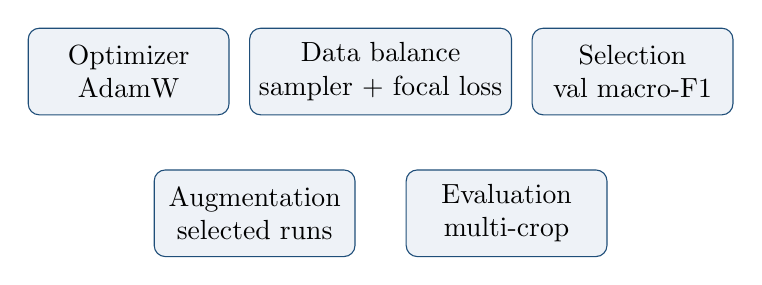
\begin{tikzpicture}[
  card/.style={draw=AccentBlue, rounded corners=4pt, fill=SoftGray, minimum width=2.55cm, minimum height=1.1cm, align=center}
]
\node[card] (a) at (0,0) {Optimizer\\AdamW};
\node[card] (b) at (3.2,0) {Data balance\\sampler + focal loss};
\node[card] (c) at (6.4,0) {Selection\\val macro-F1};
\node[card] (d) at (1.6,-1.8) {Augmentation\\selected runs};
\node[card] (e) at (4.8,-1.8) {Evaluation\\multi-crop};
\end{tikzpicture}
}
\end{columns}
\end{frame}

\begin{frame}{Results: Model Comparison}
\framesubtitle{Residual CNN is the best reported model on the saved validation and test artifacts.}
\begin{columns}[T,totalwidth=\textwidth]
\column{0.60\textwidth}
\centering
\scriptsize
\begin{tabular}{lcccc}
\toprule
Model & Val F1 & Test Acc & Test Rec & Test F1 \\
\midrule
standard\_base & 0.3624 & 0.5352 & 0.4180 & 0.3536 \\
residual & \textbf{0.5733} & \textbf{0.6780} & \textbf{0.5974} & \textbf{0.5909} \\
standard+aug & 0.4141 & 0.5511 & 0.4771 & 0.4009 \\
\bottomrule
\end{tabular}
\vspace{0.15cm}

\smallnote{Residual test macro-precision: \textbf{0.6135}}

\column{0.40\textwidth}

\includegraphics[width=\linewidth]{/Users/nisaljinadasa/Documents/Coding/genredetection/docs/model_comparison_metrics.png}
\end{columns}
\end{frame}

\begin{frame}{Results Interpretation and Error Patterns}
\framesubtitle{Global accuracy is not enough; the confusion structure shows where the model still fails.}
\begin{columns}[T,totalwidth=\textwidth]
\column{0.44\textwidth}
\begin{itemize}
  \item The residual CNN is strongest and most stable across validation and test.
  \item Macro-F1 is the key metric because minority genres are harder than major classes.
  \item Weighted metrics are higher, which indicates imbalance is still masking some failures.
  \item Error analysis should focus on confusions between semantically adjacent genres.
\end{itemize}

\column{0.56\textwidth}
\centering
\placeholderbox{0.92\linewidth}{2.5cm}
\smallnote{Insert confusion matrix screenshot}
\vspace{0.2cm}

\placeholderbox{0.92\linewidth}{1.2cm}
\smallnote{Insert per-class failure examples}
\end{columns}
\end{frame}

\begin{frame}{Demo Architecture and User Flow}
\framesubtitle{The later demo is a deployment prototype, with its own model and UI path.}
\begin{columns}[T,totalwidth=\textwidth]
\column{0.42\textwidth}
\begin{itemize}
  \item User uploads audio or selects a sample in the frontend.
  \item The frontend sends the file to a FastAPI backend.
  \item The API preprocesses audio, runs inference, and returns top predictions.
  \item The UI renders ranked genres and confidence bars.
  \item This demo uses a later trained model, so its metrics are reserved separately from the main benchmark story.
\end{itemize}

\column{0.58\textwidth}
\centering
\resizebox{\linewidth}{!}{
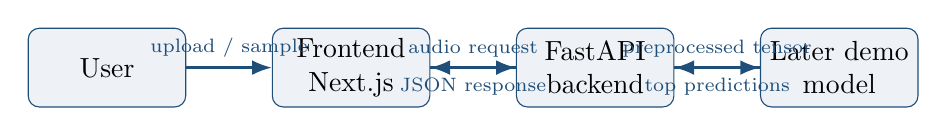
\begin{tikzpicture}[
  actor/.style={draw=AccentBlue, rounded corners=4pt, fill=SoftGray, minimum width=2.0cm, minimum height=1.0cm, align=center},
  arr/.style={-{Latex[length=2.5mm]}, thick, AccentBlue}
]
\node[actor] (u) at (0,0) {User};
\node[actor] (f) at (3.1,0) {Frontend\\Next.js};
\node[actor] (a) at (6.2,0) {FastAPI\\backend};
\node[actor] (m) at (9.3,0) {Later demo\\model};
\draw[arr] (u) -- node[above, font=\scriptsize] {upload / sample} (f);
\draw[arr] (f) -- node[above, font=\scriptsize] {audio request} (a);
\draw[arr] (a) -- node[above, font=\scriptsize] {preprocessed tensor} (m);
\draw[arr] (m) -- node[below, font=\scriptsize] {top predictions} (a);
\draw[arr] (a) -- node[below, font=\scriptsize] {JSON response} (f);
\end{tikzpicture}
}
\vspace{0.25cm}

\placeholderbox{0.92\linewidth}{1.1cm}
\smallnote{Insert later-model metrics here}
\end{columns}
\end{frame}

\begin{frame}{Demo Walkthrough}
\framesubtitle{Use screenshots here to show the full request-response path end to end.}
\begin{columns}[T,totalwidth=\textwidth]
\column{0.40\textwidth}
\begin{enumerate}
  \item Pick a sample track or upload a new file.
  \item Backend resamples, trims or pads, and computes features.
  \item The model returns top-K predicted genres.
  \item The frontend renders confidence bars for interpretation.
\end{enumerate}
\smallnote{Use this slide to transition cleanly into the live demo.}

\column{0.60\textwidth}
\centering
\begin{tabular}{cc}
\placeholderbox{2.7cm}{1.4cm} &
\placeholderbox{2.7cm}{1.4cm} \\
\smallnote{Landing page} & \smallnote{Selected sample / upload} \\
\placeholderbox{2.7cm}{1.4cm} &
\placeholderbox{2.7cm}{1.4cm} \\
\smallnote{Prediction bars} & \smallnote{API / network flow} \\
\end{tabular}
\end{columns}
\end{frame}

\begin{frame}{Limitations and Risks}
\framesubtitle{These are the main reasons the model can still be wrong even when the pipeline is correct.}
\begin{columns}[T,totalwidth=\textwidth]
\column{0.46\textwidth}
\begin{itemize}
  \item Genre labels are noisy and sometimes ambiguous.
  \item Class imbalance still hurts minority-genre performance.
  \item Adjacent genres remain a major source of confusion.
  \item The main evaluated model and later demo model are not the same artifact.
\end{itemize}

\column{0.54\textwidth}
\centering
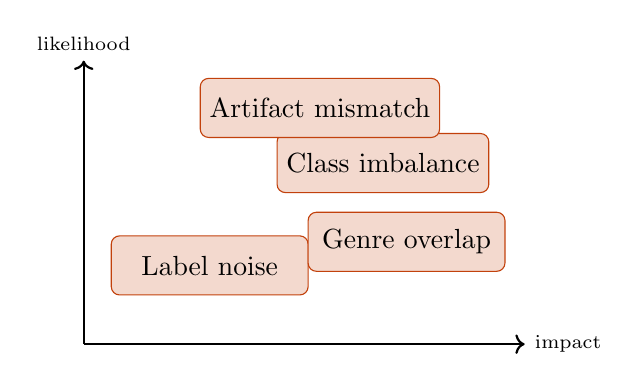
\begin{tikzpicture}[
  axis/.style={font=\scriptsize},
  risknode/.style={draw=AccentOrange, fill=AccentOrange!20, rounded corners=3pt, minimum width=2.5cm, minimum height=0.75cm, align=center}
]
\draw[->, thick] (0,0) -- (5.6,0) node[right, axis] {impact};
\draw[->, thick] (0,0) -- (0,3.6) node[above, axis] {likelihood};
\node[risknode] at (1.6,1.0) {Label noise};
\node[risknode] at (3.8,2.3) {Class imbalance};
\node[risknode] at (4.1,1.3) {Genre overlap};
\node[risknode] at (3.0,3.0) {Artifact mismatch};
\end{tikzpicture}
\end{columns}
\end{frame}

\begin{frame}{Conclusion and Next Steps}
\framesubtitle{The work is complete as a pipeline, but the demo and model governance can still be tightened.}
\begin{columns}[T,totalwidth=\textwidth]
\column{0.48\textwidth}
\begin{itemize}
  \item We built a reproducible audio ML pipeline from dataset curation to inference.
  \item The residual CNN is the best reported model in the main benchmark story.
  \item The later demo model shows a practical path toward interactive deployment.
\end{itemize}
\vspace{0.3cm}
\begin{block}{Next Step}
Unify the production demo with the best evaluated checkpoint and report its deployment metrics.
\end{block}

\column{0.52\textwidth}
\centering
\resizebox{\linewidth}{!}{
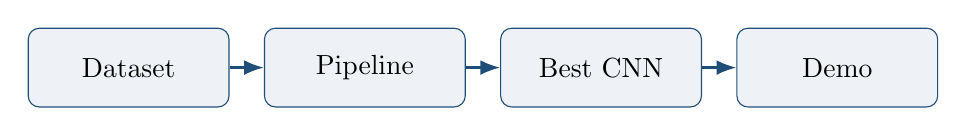
\begin{tikzpicture}[
  box/.style={draw=AccentBlue, rounded corners=4pt, fill=SoftGray, minimum width=2.55cm, minimum height=1.0cm, align=center},
  arr/.style={-{Latex[length=2.5mm]}, thick, AccentBlue}
]
\node[box] (a) at (0,0) {Dataset};
\node[box] (b) at (3.0,0) {Pipeline};
\node[box] (c) at (6.0,0) {Best CNN};
\node[box] (d) at (9.0,0) {Demo};
\draw[arr] (a) -- (b);
\draw[arr] (b) -- (c);
\draw[arr] (c) -- (d);
\end{tikzpicture}
}
\end{columns}
\end{frame}

\end{document}
